%
% Portuguese-BR vertion
% 
\documentclass{article}

\usepackage{ipprocess}
% Use longtable if you want big tables to split over multiple pages.
% \usepackage{longtable}
\usepackage[utf8]{inputenc} 
\usepackage[brazil]{babel} % Uncomment for portuguese

\sloppy

\graphicspath{{./pictures/}} % Pictures dir
\makeindex
\begin{document}

\DocumentTitle{Documento de Casos de Uso}
\Project{Core-MUSA}
\Organization{Universidade Estadual de Feira de Santana}
\Version{Build 3}

\capa
\newpage

%%%%%%%%%%%%%%%%%%%%%%%%%%%%%%%%%%%%%%%%%%%%%%%%%%
%% Revision History
%%%%%%%%%%%%%%%%%%%%%%%%%%%%%%%%%%%%%%%%%%%%%%%%%%
\section*{\center Histórico de Revisões}
  \vspace*{1cm}
  \begin{table}[ht]
    \centering
    \begin{tabular}[pos]{|m{2cm} | m{7.2cm} | m{3.8cm}|} 
      \hline
      \cellcolor[gray]{0.9}
      \textbf{Date} & \cellcolor[gray]{0.9}\textbf{Descrição} & \cellcolor[gray]{0.9}\textbf{Autor(s)}\\ \hline
      \hline
      \small 08/10/2014 & \small Concepção do documento & \small 
      \begin{itemize}
      	\item bezourokq;
      	\item wsbittencourt;
      	\item fmbboaventura;  
	  \end{itemize}      	
      \\ \hline
      \small 13/10/2014 & \small Build 2: Novo modelo de caso de uso & \small 
      \begin{itemize}
      	\item wsbittencourt;
      	\item jadsonfirmo;
      	\item fmbboaventura;  
	  \end{itemize}      	
      \\ \hline
      \small 16/10/2014 & \small Build 3: Novo modelo de caso de uso & \small 
      \begin{itemize}
      	\item wsbittencourt; 
	  \end{itemize} 
	  \\ \hline
      \small 20/10/2014 & \small Adição caso de uso LW e SW & \small 
      \begin{itemize}
      	\item kelvincarmo; 
	  \end{itemize} 
	  \\ \hline
	  \small 23/10/2014 & \small Revisão & \small 
      \begin{itemize}
      	\item jadsonfirmo; 
	  \end{itemize}  
	  \\ \hline
	  
	  \small 29/10/2014 & \small Inclusão Casos de Uso: JPC & \small 
	  \begin{itemize}
	  	\item di3goleite; 
	  \end{itemize}  
	  \\ \hline
	  
	  \small 29/10/2014 & \small Inclusão Casos de Uso: RET e NOP & \small 
      \begin{itemize}
      	\item mtcastro; 
	  \end{itemize}  
	  \\ \hline
	  
	  \small 30/10/2014 & \small Refatoração do documento & \small 
	  \begin{itemize}
	  	\item di3goleite; 
	  \end{itemize}  
	  \\ \hline
	  	 
	  \small 30/10/2014 & \small Inclusão Casos de Uso: HALT & \small 
      \begin{itemize}
      	\item mtcastro; 
	  \end{itemize}
 	   \\ \hline

 	 \small 30/10/2014 & \small Refatoração dos fluxos e tamanho das Imagens & \small 
      \begin{itemize}
      	\item Odivio Caio; 
	  \end{itemize}
	  \\ \hline

	\small 12/12/2014 & \small Adição dos novos casos de uso& \small 
      \begin{itemize}
      	\item Odivio Caio; 
	  \end{itemize}
	  
	  \\ \hline
    \end{tabular}
  \end{table}

\newpage

% TOC instantiation
\tableofcontents
\newpage

%%%%%%%%%%%%%%%%%%%%%%%%%%%%%%%%%%%%%%%%%%%%%%%%%%
%% Document main content
%%%%%%%%%%%%%%%%%%%%%%%%%%%%%%%%%%%%%%%%%%%%%%%%%%
\section{Introdução}
Este documento tem como objetivo a especificação dos casos de uso do projeto Core Musa (concepção de um processador simples de propósito geral). O documento detalha cada caso de uso indicando os atores, os eventos (ações) e as condições de cada caso, além dos diagramas de casos de uso.

  \subsection{Objetivo}
  
  \subsection{Visão Geral do Documento}
  \begin{itemize}
    \item Sessão 2: Lista todos os possíveis atores do sistema.
    \item Sessão 3: Relata a lista dos casos de uso do projeto.
    % \item Referências: provê uma lista completa de todos os artefatos referenciados nesse documento.
  \end{itemize}
  
  \subsection{Representação Simbólica}
  A Figura \ref{fig:uc_exemple} ilustra a simbologia utilizada para representar operações que devem ser realizadas pelo sistema. A Figura \ref{fig:actors} apresenta os modelos de ilustração utilizados para representar os Atores do sistema. Um ator, dentro do escopo desta descrição, pode ser identificado como um módulo \textit{top level}, ou como um elemento de entrada e saída (botões, sensores, \textit{displays}, etc).
  
  \FloatBarrier
  \begin{figure}[H]
    \centering
    
\includegraphics[width=0.25\textwidth]{uc_exemple.png}
    \caption{Exemplo de Caso de Uso.}
    \label{fig:uc_exemple}
  \end{figure}
  
  A simbologia usual para representação de um Ator é apresentada na Figura \ref{fig:actor_exemple}, no entanto, para representar módulos incorporados, utiliza-se as representações ilustradas nas Figuras \ref{fig:ipcore_exemple} e \ref{fig:ipcore_single_exemple}, definidas por convenção. Este elemento, em geral, está associado aos módulos do sistema, ou IP cores de terceiros incorporados ao mesmo. Esta simbologia foi divida, com o objetivo de representar instâncias únicas (Figura \ref{fig:ipcore_single_exemple}), ou múltiplas (Figura \ref{fig:ipcore_exemple}) de um determinado componente. 
  
  \FloatBarrier
  \begin{figure}[H]
    \centering
    \begin{subfigure}[b]{0.3\textwidth}
      \centering
      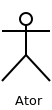
\includegraphics[width=0.25\textwidth]{actor_exemple.png}
      \caption{Ator do Sistema.}
      \label{fig:actor_exemple}
    \end{subfigure} 
    \begin{subfigure}[b]{0.3\textwidth}
      \centering
      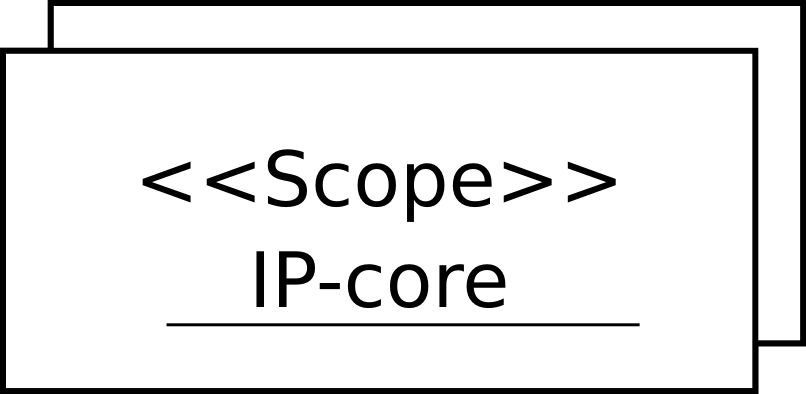
\includegraphics[width=0.6\textwidth]{ipcore_exemple.png}
      \caption{Instância múltipla de um IP.}
      \label{fig:ipcore_exemple}
    \end{subfigure}
    \begin{subfigure}[b]{0.3\textwidth}
      \centering
      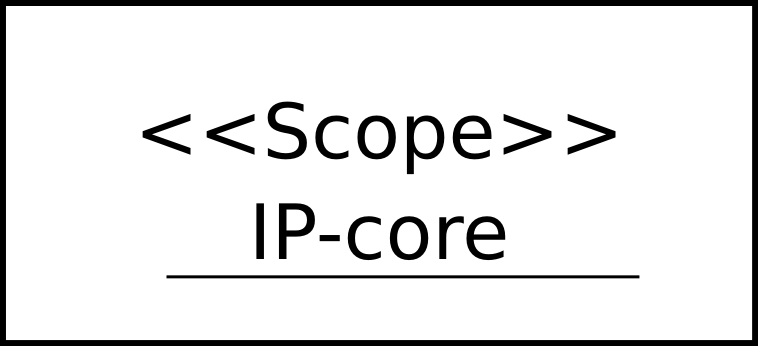
\includegraphics[width=0.6\textwidth]{ipcore_single_exemple.png}
      \caption{Instância de um IP.}
      \label{fig:ipcore_single_exemple}
    \end{subfigure}
    \caption{Simbologia utilizada na implementação dos Casos de Uso.}
    \label{fig:actors}
  \end{figure}
  
  O projetista responsável por interpretar os diagramas não deve confundir-se no momento de analisar as simbologias de atores. A representação alternativa, não implica que o módulo será instanciado no subsistema em questão, mas sim que os recursos providos por este \textit{core} são necessários para garantir o seu funcionamento.
  
  \subsection{Definições, Acrônimos e Abreviações}
  \FloatBarrier
    \begin{table}[H] 
      \begin{center}
        \begin{tabular}[pos]{|m{2cm} | m{8cm}|} 
          \hline 
          \cellcolor[gray]{0.9}\textbf{Termo} & \cellcolor[gray]{0.9}\textbf{Descrição} \\ \hline
          UC & Caso de Uso  \\ \hline
          ULA & Unidade Lógica e Aritmética \\ \hline
          NFR & Requisito Não Funcional \\ \hline
          FR & Requisito Funcional \\ \hline
	BR & Banco de Registradores \\ \hline
          PC & \textit{Program Counter} \\
          \hline
        \end{tabular}
      \end{center}
    \label{tab:definicoes}
    \end{table}

  \section{Atores do Sistema}
  
\begin{figure}[htb]
\centering
\begin{minipage}[c]{0.19\linewidth}
\centering
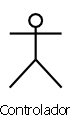
\includegraphics[scale=0.50]{./pictures/use/atores/controlador.png}
\end{minipage}
\begin{minipage}[c]{0.19\linewidth}
\centering

\includegraphics[scale=0.50]{./pictures/use/atores/ula.png}
\end{minipage}
\end{figure}

\textbf{Controlador} – Unidade que controla a execução das operações.

\textbf{ULA} – Unidade L\'{o}gica e Aritm\'{e}tica.
  
  \section{Casos de Usos}
  Esta sessão apresenta o conjunto de UC realizados para a implementação do projeto \textit{Core }MUSA (Núcleo de processamento de instruções do processador de propósito geral MUSA). As sessões a seguir foram divididas e nomeada utilizando a nomenclatura abreviada [UC (NÚMERO DO UC)] seguido de uma breve descrição em forma de título.

 \usecase{Execução de instruções}
  O controlador deve ser capaz de decodificar a instrução e operá-la no sistema.
  
  \actors
    \begin{description}
     \item \textbf{Controlador}.
    \end{description}
    
  \preconditions 
    \begin{itemize}
     \item Endereço apotado por PC ser válido;
     \item instrução possuir um \textit{OPCODE} válido;
    \end{itemize}

  \postconditions
    \begin{itemize}
     \item Execução da Instrução.
    \end{itemize}

   \ucdiagram{./pictures/use/case/decodificacao.png}
  
  % descricao do fluxo principal de eventos
  \begin{mainflow}
    \item Controlador faz a decodificação do \textit{opcode} da instrução recebida;
  \end{mainflow}

    \usecase{Instruções  L\'{o}gicas e Aritm\'{e}ticas.}
  A ULA é responsável por efetuar as operações Logicas e Aritiméticas.
  
  \actors
    \begin{description}
     \item \textbf{ULA} .
    \end{description}
    
  \preconditions 
    \begin{itemize}
     \item Atender aos requisitos funcionais [FR03 a FR10];
     \item Endereço(s) do(s) registradores serem válidos;
    \end{itemize}

  \postconditions
    \begin{itemize}
     \item Ter como saida o Valor resultante e a  \textit{Flag}, caso ocorra.
    \end{itemize}
  
  \ucdiagram{./pictures/use/case/NewUla.png}
  
  % descricao do fluxo principal de eventos
  \begin{mainflow}
    \item Realização da ação referente ao \textit{Function} recebido;
    \item \textit{Flags} são disparadas, caso seja necessário;
    \item Apresentação do resultado;
  \end{mainflow}

\usecase{Desvios}
   O processador tem a capacidade de desviar do fluxo normal de execução.
  
  \actors
    \begin{description}
     \item \textbf{Controlador}.
    \end{description}
    
  \preconditions 
    \begin{itemize}
     \item Endereço do saltor ser válido;
    \end{itemize}

  \postconditions
    \begin{itemize}
     \item Modificação do PC.
    \end{itemize}

  \ucdiagram{./pictures/use/case/jump.png}
  
  % descricao do fluxo principal de eventos
  \begin{mainflow}
    \item Controlador executa a escrita no PC;
  \end{mainflow}  

\usecase{Leitura e Escrita no BR}
   O processador tem a capacidade de efetuar a leitura ou escrita de um valor de 32 bits no Banco de Registradores.
  
  \actors
    \begin{description}
     \item \textbf{Controlador}.
    \end{description}
    
  \preconditions 
    \begin{itemize}
    \item Sinais de Controle;
    \item Endereço(s) do(s) registrador(s);
    \end{itemize}

  \postconditions
    \begin{itemize}
    \item Saidas de 32 bits.
    \end{itemize}

  \ucdiagram{./pictures/use/case/BD.png}
  
  % descricao do fluxo principal de eventos
  \begin{mainflow}
    \item Controlador executa a leitura ou a escrita no Banco de Registradores;
    \item O modulo BR identifica os endereços e apresenta as saidas;
  \end{mainflow}  

\usecase{Imediatos do tipo aritmético e lógico}
   O sistema tem a capacidade de enviar valores imediatos para ULA.
  
  \actors
    \begin{description}
     \item \textbf{Controlador}.
     \item \textbf{ULA}.
    \end{description}
    
  \preconditions 
    \begin{itemize}
    \item Sinais de Controle;
    \end{itemize}

  \postconditions
    \begin{itemize}
    \item Saidas de 35 bits.
    \end{itemize}

  \ucdiagram{./pictures/use/case/ImeArit.png}
  
  % descricao do fluxo principal de eventos
  \begin{mainflow}    \item Realização da ação referente ao \textit{Function} recebido;
    \item Valor imediato recebido é estendido;
    \item \textit{Flags} são disparadas, caso seja necessário;
    \item Apresentação do resultado;
  \end{mainflow}  
 

% Optional bibliography section
% To use bibliograpy, first provide the ipprocess.bib file on the root folder.
% \bibliographystyle{ieeetr}
% \bibliography{ipprocess}

\end{document}
